\section{The Spartan Protocol}\label{sec:spartan}

\subsection{Preliminaries}

The Spartan protocol is designed to prove the satisfiability of Rank-1 Constraint System (R1CS).
An R1CS instance is defined by a set of matrices $(A, B, C)$ over a field $\mathbb{F}$ (more generally the definition makes sense over any semiring $\mathsf{R}$), and it is satisfied by a public input $x$ and a private witness $w$ if the combined vector $z = (x, w)$ satisfies the relation:
\[ (A \cdot z) \circ (B \cdot z) = (C \cdot z) \]
where $\circ$ denotes the Hadamard (entry-wise) product.
Our formalization follows the definition in \texttt{ArkLib/ProofSystem/ConstraintSystem/R1CS.lean}.

\subsection{Description in Paper}

\Cref{fig:spartan_protocol} is the description of the Spartan protocol from the original
paper~\cite{spartan}. Note that in this section, we only formalize the \emph{Polynomial IOP (PIOP)}
aspect of Spartan. In the PIOP model, the prover does not commit to polynomials using a Polynomial
Commitment Scheme (PCS). Instead, the verifier is given oracle access to the polynomials. Therefore,
steps involving `PCS.Setup`, `PCS.Commit`, and `PCS.Eval` are replaced by simple oracle interactions.

\begin{figure}[ht]
    \centering
    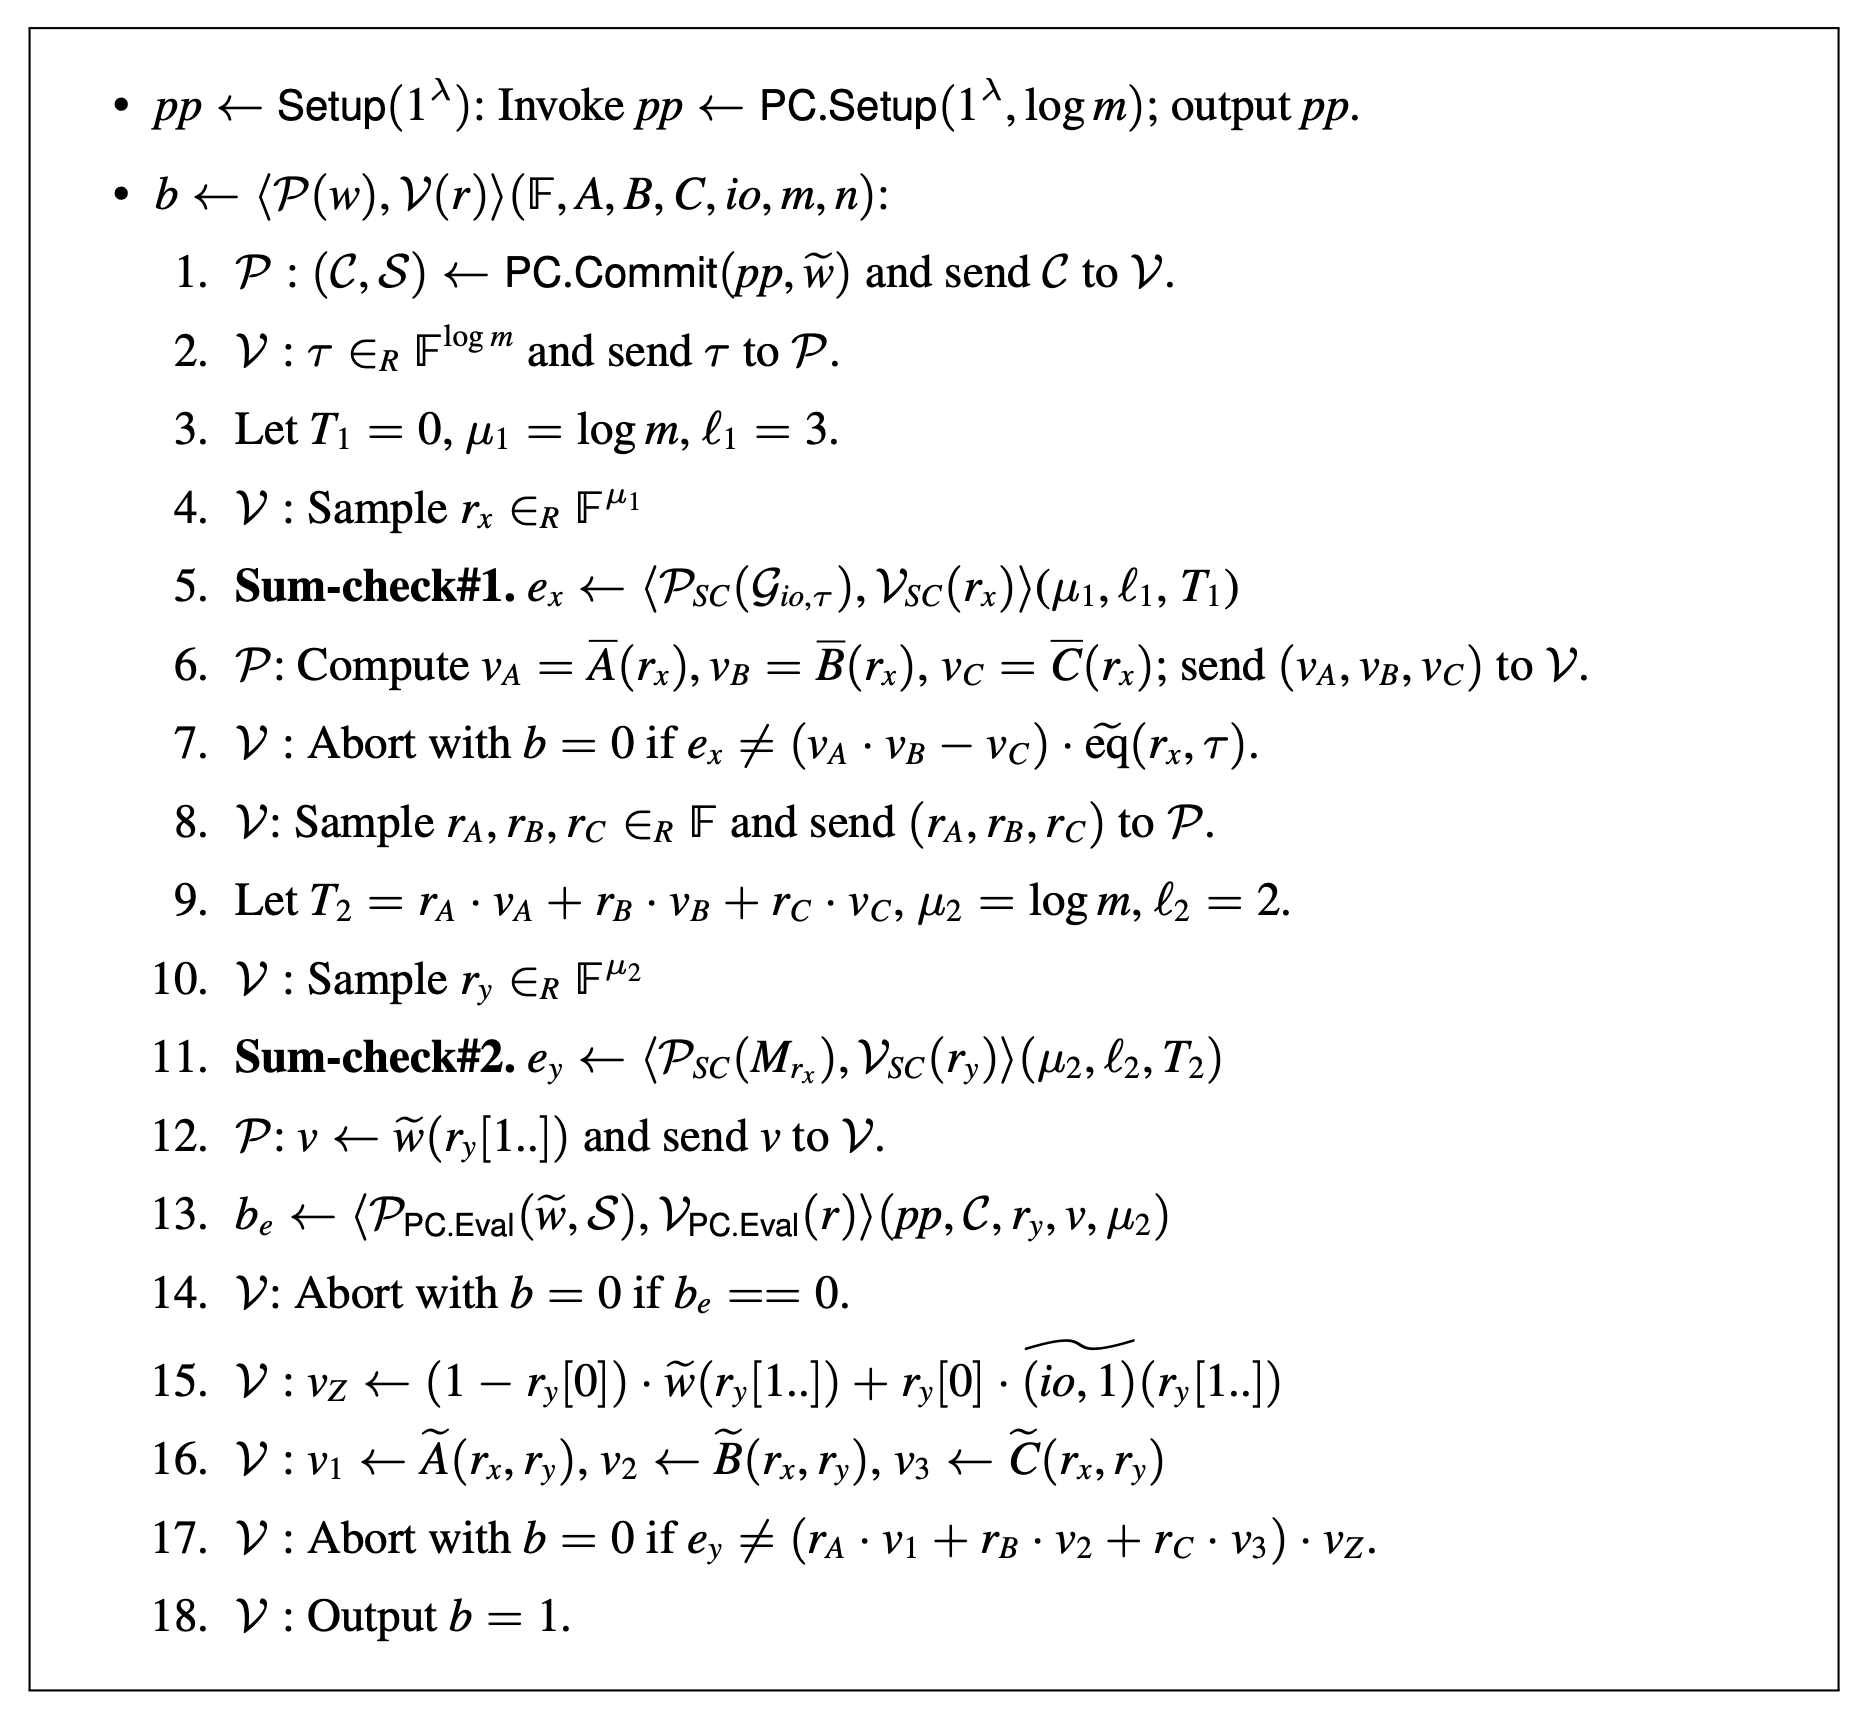
\includegraphics{figures/spartan-description.png}
    \caption{The Spartan protocol description, from the original paper.}
    \label{fig:spartan_protocol}
\end{figure}

After stripping away the polynomial commitment scheme, the protocol has the following structure:

\begin{description}
    \item[Setup:] This step is part of the polynomial commitment scheme and is not part of the PIOP we formalize.
    \item[Interaction:] The interaction is between a prover $\mathcal{P}$ with witness $w$ and a verifier $\mathcal{V}$ with public inputs $(\mathbb{F}, A, B, C, \text{io}, m, n)$.
    \begin{enumerate}
        \item $\mathcal{P}$: Sends oracle access to the multilinear extension of the witness, $\tilde{w}$, to $\mathcal{V}$. In the original paper, this is a commitment $(C,S) \leftarrow \text{PC.Commit}(\text{pp}, \tilde{w})$.
        \item $\mathcal{V}$: Samples a random challenge $\tau \in \mathbb{F}^{\log m}$ and sends it to $\mathcal{P}$.
        \item Let $T_1 = 0$, $\mu_1 = \log m$, $\ell_1 = 3$. These are parameters for the first sum-check protocol.
        \item $\mathcal{V}$: Samples a random challenge $r_x \in \mathbb{F}^{\mu_1}$.
        \item \textbf{Sum-check\#1.} A sum-check protocol is executed. The verifier receives the claimed evaluation $e_x$. The prover of the sum-check has oracle access to a polynomial $G_{io, \tau}$, and the verifier has oracle access to $r_x$. The parameters for this sub-protocol are $(\mu_1, \ell_1, T_1)$.
        \item $\mathcal{P}$: Computes evaluations $v_A = \tilde{A}(r_x)$, $v_B = \tilde{B}(r_x)$, $v_C = \tilde{C}(r_x)$ and sends them to $\mathcal{V}$. $\tilde{A}, \tilde{B}, \tilde{C}$ are multilinear extensions of the matrices $A, B, C$.
        \item $\mathcal{V}$: Aborts if $e_x \neq (v_A \cdot v_B - v_C) \cdot \tilde{\text{eq}}(r_x, \tau)$. This is the verifier's check for the first sum-check.
        \item $\mathcal{V}$: Samples random challenges $r_A, r_B, r_C \in \mathbb{F}$ and sends them to $\mathcal{P}$.
        \item Let $T_2 = r_A \cdot v_A + r_B \cdot v_B + r_C \cdot v_C$, $\mu_2 = \log n$, $\ell_2 = 2$. These are parameters for the second sum-check protocol. Note: The image states $\mu_2 = \log m$, which is likely a typo and should be $\log n$.
        \item $\mathcal{V}$: Samples a random challenge $r_y \in \mathbb{F}^{\mu_2}$.
        \item \textbf{Sum-check\#2.} Another sum-check protocol is executed. The verifier receives the claimed evaluation $e_y$.
        \item $\mathcal{P}$: Computes $v \leftarrow \tilde{w}(r_y[1..])$ and sends $v$ to $\mathcal{V}$.
        \item This step involves a polynomial commitment evaluation proof. In our PIOP formalization, this check is not needed as the verifier has direct oracle access to $\tilde{w}$.
        \item $\mathcal{V}$: This step is part of the evaluation proof check, so it is omitted.
        \item $\mathcal{V}$: Computes $v_Z \leftarrow (1 - r_y[0]) \cdot \tilde{w}(r_y[1..]) + r_y[0] \cdot \widetilde{(\text{io}, 1)}(r_y[1..])$. This reconstructs the evaluation of the combined input-witness vector polynomial $\tilde{z}$.
        \item $\mathcal{V}$: Queries oracles for $\tilde{A}, \tilde{B}, \tilde{C}$ at $(r_x, r_y)$ to get $v_1, v_2, v_3$.
        \item $\mathcal{V}$: Aborts if $e_y \neq (r_A \cdot v_1 + r_B \cdot v_2 + r_C \cdot v_3) \cdot v_Z$. This is the final check.
        \item $\mathcal{V}$: Outputs 1.
    \end{enumerate}
\end{description}

\subsection{Formalization using IOR Composition}
